\documentclass[a4paper, 12pt, fleqn]{report}

% - - - - -

% Packages
\usepackage[utf8]{inputenc}
\usepackage[english]{babel} % Hyphenation
\usepackage{graphicx,csquotes} % Images
\usepackage[nodisplayskipstretch]{setspace}
\setstretch{1.5} % 1.5 interline
\usepackage[left=2.5cm, right=2.5cm, top=2.54cm, bottom=2.54cm]{geometry}
\usepackage{amsmath,amssymb}
\usepackage{mathtools}
\usepackage[hidelinks]{hyperref}
\usepackage{multicol}
\usepackage[style=authoryear,maxcitenames=2]{biblatex}
\addbibresource{bibliography.bib}
\usepackage{tablefootnote}
\usepackage{blindtext}
\usepackage{caption}
\usepackage[toc]{appendix}
%\usepackage{times} % Font Times New Roman
%\usepackage{showframe} % Show page margins

\newcommand{\charactercount}[1]{
\immediate\write18{
    expr `texcount -1 -sum -merge #1.tex` + `texcount -1 -sum -merge -char #1.tex` - 1 
    > chars.txt
}\input{chars.txt}}

\usepackage[T1]{fontenc}
\usepackage{titlesec, color}
\definecolor{gray75}{gray}{0.75}
\newcommand{\hsp}{\hspace{20pt}}
\titleformat{\chapter}[hang]{\Huge\bfseries}{\thechapter\hsp\textcolor{gray75}{|}\hsp}{0pt}{\Huge\bfseries}
\titlespacing*{\chapter}{0pt}{-50pt}{40pt}

\newcommand\scalemath[2]{\scalebox{#1}{\mbox{\ensuremath{\displaystyle #2}}}}

% - - - - -

\begin{document}

\begin{titlepage}

\begin{center}
    {\large \uppercase{\textbf{Ludwig-Maximilians-Universität München}}}

    \vspace{0.5cm}
    
    {\Large Department of Economics}
    
    \vspace{0.5cm}

    {\Large Seminar "Tax Policy and Multinational Firms"}

    \vspace{0.5cm}

    {\Large Summer Semester 2023}
\end{center}

\vspace{0.5cm}

\begin{figure}[h]
    \centering
    
\includegraphics[width=95pt]{img/lmu-logo.png}
\end{figure}

\begin{center}
    {\Large \textbf{Countries Do Compete over Corporate Tax Rates\\while Keeping Revenues Stable}\par}
\end{center}

\vfill

\begin{multicols}{2}
\noindent\large \textbf{Student}\\
\large Giovanni Remonti\\
\large giovanni.remonti@campus.lmu.de\\
\large Matrikel-Nr. 12621881\\
\large Second Semester

\columnbreak

\begin{flushright}
\large \textbf{Supervisor}\par
\large Jelena Todorović Bojović\par
\end{flushright}
\end{multicols}

\end{titlepage}

\tableofcontents

%\charactercount{main}

\chapter{Introduction}

Climate change and its consequences are one of the greatest challenges of our time. Human activities, with the emission of greenhouse gases, have unequivocally caused global warming \parencite{IPCC2023}.  To keep global warming within a manageable path, numerous mitigation and adaptation actions and policies are needed. If applied on a large scale, economic instruments can also help reduce emissions, and among these, carbon taxes and their various implementations play an important role. As the report of \textcite{IPCC2023} reveals, in 2020, over 20\% of global greenhouse gas emissions were covered by carbon taxes or Emission Trading Systems. These instruments have proven to be effective in reducing emissions and, in addition, carbon tax revenues are often redistributed to low-income households to address equity issues.

In this context, \textcite{Larch2017} study the impacts of introducing carbon tariffs on trade flows, welfare, and emissions. To do so, they implement a widely used framework in the international trade literature, such as a structural gravity model. Moreover, taking advantage of the work of \textcite{copeland2005}, they are also the first to isolate the effects that influence emissions in this framework. Not only this, \textcite{Larch2017} also assess the rate of carbon leakage that arises when only a subset of countries commit to their climate commitments, with and without carbon tariffs.

This seminar paper proceeds as follows: Chapter \ref{sec:theorethical} summarizes the paper of \textcite{Larch2017}, Chapter \ref{sec:literature} reviews the literature on carbon tariffs and compares results, Chapter \ref{sec:extension} proposes two extensions to the paper of \textcite{Larch2017}, Chapter \ref{sec:conclusion} concludes.
\chapter{The impact of soft-skills training for entrepreneurs in Jamaica }
\label{sec-2-summary}

Jamaica, an island in the Greater Antilles, is a Commonwealth realm with a population of over 2.8 million people. Since its independence in 1962, the country has experienced a modest growth mainly driven by the services and tourism sectors. Today, Jamaica registers a low unemployment rate of around 6\%, offset by the lowest ever total factor productivity \parencite{WorldBank}.

In this context, \cite{Ubfal2022} set up a Randomized Control Trial (RCT) to test the impacts (i.e., causal effects) of two different types of business training programs on small entrepreneurs and their business outcomes. The authors worked together with the Jamaica Business Development Corporation (JBDC), a governmental organization, which was in charge of delivering the training programs. This Section presents the paper and its findings, highlighting in particular the effectiveness of soft-skills training in fostering the adoption of recommended business practices.



\section{Methodology}

\subsection{Training Programs}

Together with JBDC, the research team developed and adapted for the local context two training programs, which represent the two treatments. Both were taught by the same teachers in the same facilities over 10 weeks, and both had the same duration, 40 hours, split into two parts, where the second half differentiated each program. The lectures took place between October and December 2016.

During the first common 5 weeks, the lectures aimed to develop personal initiative in the participants. A choice motivated by the notion that a proactive trait is essential for entrepreneurs to be able to anticipate and prepare for potential opportunities and threats \parencite{Frese2014}.

In the remaining weeks, the combined training expanded its contents to typical business training topics, such as financial management or marketing. Instead, the soft-skills training provided more materials related to personal initiative, such as perseverance and problem solving. This different approach, which includes insights from the psychology literature, is the real focus of the following analysis because the authors are interested in assessing whether practicing more the participants' soft-skills is more beneficial, in terms of business outcomes, than simply discussing business practices.

\subsection{Sampling and Randomization}

\begin{table}
\centering
\caption{Baseline Balance (extract), \cite{Ubfal2022}}
\label{sum-baseline-balance}
\begin{adjustbox}{width=\textwidth}
\begin{tabular}{lccccc}
\toprule
                                                                                                      & Control group (C) & Soft-skills training (T1) & Combined training (T2) & T1 = C               & T2 = C                \\
                                                                                                      & Mean              & Mean                      & Mean                   & P-val.               & P-val.                \\ 
\hline
\textbf{Panel A. Stratification variables}                                                            &                   &                           &                        &                      &                       \\
Female                                                                                                & 0.58              & 0.59                      & 0.58                   & 0.87                 & 1.00                  \\
Has employees                                                                                         & 0.30              & 0.30                      & 0.30                   & 0.86                 & 0.91                  \\
Education: more secondary                                                                             & 0.61              & 0.61                      & 0.60                   & 0.87                 & 0.81                  \\
\textbf{Panel B. Owner characteristics}                                                               &                   &                           &                        &                      &                       \\
Age                                                                                                   & 42.43             & 41.29                     & 42.20                   & 0.22                 & 0.81                  \\
Black                                                                                                 & 0.90              & 0.92                      & 0.91                   & 0.39                 & 0.53                  \\
Married                                                                                               & 0.46              & 0.39                      & 0.44                   & 0.06                 & 0.62                  \\
Set a goal for business                                                                               & 0.84              & 0.85                      & 0.84                   & 0.77                 & 0.81                  \\
Wants to channge sth                                                                                  & 0.64              & 0.63                      & 0.68                   & 0.92                 & 0.27                  \\
Personal initiative                                                                                   & 6.01              & 6.01                      & 6.07                   & 0.99                 & 0.32                  \\
\textbf{Panel C. Firm characteristics}                                                                &                   &                           &                        &                      &                       \\
Keeps formal accounts                                                                                 & 0.08              & 0.09                      & 0.13                   & 0.59                 & 0.03                  \\
Registered business                                                                                   & 0.53              & 0.51                      & 0.54                   & 0.72                 & 0.69                  \\
Sales in the last month                                                                               & 87766             & 100744                    & 75922                  & 0.47                 & 0.42                  \\
Business practice index                                                                               & 0.58              & 0.59                      & 0.61                   & 0.57                 & 0.18                  \\ 
\hline
\begin{tabular}[c]{@{}l@{}}\textbf{Panel D. Aggr. Orthog. test}\\\textbf{for~panels B-C}\end{tabular} &                   &                           &                        &                      &                       \\
P-value                                                                                               &                   &                           &                        & 0.91                 & 0.52                  \\ 
\hline
Observations                                                                                          & 315               & 315                       & 315                    & \multicolumn{1}{l}{} & \multicolumn{1}{l}{}\\
\bottomrule 
\end{tabular}
\end{adjustbox}
\end{table}

Entrepreneurs were recruited through a telemarketing campaign. At first, around 2000 business owners living in Kingston and surroundings expressed their interest in the program. Secondly, to gather information about the participants and their businesses, a baseline survey was given to the contacts. To reduce heterogeneity and create more comparable groups, the authors established certain eligibility criteria, such as having fewer than five employees and reporting less than JMD 1 million in monthly sales and costs, thus increasing the sensitivity of the analysis and drawing more reliable conclusions. The final sample included 945 entrepreneurs. Lastly, to ensure the RCT design, after a stratification based on certain variables like gender and education, business owners were randomly assigned to the two training programs, i.e. treatments, and to a control group.

Table \ref{sum-baseline-balance} summarizes the characteristics of the three groups, depicting a successful balanced randomization. In the three samples, female entrepreneurs are 58\%, the mean age is around 42 years old, and between 39\% and 46\% are married. The majority has a goal for its business (84\%) and wants to change something in it ($\sim$~64\%). On a scale of 1 to 7 (maximum), the personal initiative indicator scores 6. Half of the businesses are registered, but only a small portion keeps formal accounts ($\sim$ 9\%), and business practices are only partially widespread (59\%).

\subsection{Instruments}

To measure the impacts of the experiment on the business outcomes and a series of intermediate channels through which the treatments may interact, \cite{Ubfal2022} collected data during and after the trial with different surveys and tests.

The three main instruments are the baseline survey and the two follow-ups at 3 and 12 months, in order to capture potential short and long-term effects. The baseline survey was carried out during the sampling phase, between August and September 2016. Three months after the end of the training, in March 2017, the first follow-up survey was conducted  by a designated international survey firm. Questions related to sales, profits, business practices, and soft skills were asked. At this stage, the response rate stood at 73\% in total. In January 2018, the second follow-up took place. The same questions were asked, but the response rate stopped at 59\%. The authors explain the low participation rate in the subsequent poll by pointing out that lottery scams are very common in Jamaica and discourage people from participating in interviews, even when they are offered monetary incentives.

In addition to the ones already mentioned, class attendance was observed, and a knowledge test was given at the penultimate class. Finally, the second follow-up survey contained an additional set of questions aimed to assess specific soft-skills as well as another questionnaire designed to measure participants' grit.

\subsection{Statistical Analysis}

The RCT design chosen by \cite{Ubfal2022}, by randomly assigning participants to treatment and control groups, minimizes the selection bias and offers a robust method for determining causal relationships. In the following linear regression model, the coefficients of the treatment dummy variables represent the estimated treatment effects on the various business outcomes studied by the authors, such as firm survival, sales, and profit changes. The authors boost the statistical power using ANCOVA regressions and report intention-to-treat effects, analyzing outcomes based on initial training assignments, irrespective of actual participation. The following OLS regression is estimated:
\begin{equation}
Y_{it}=\alpha+\boldsymbol{\beta_1}T1_i+\boldsymbol{\beta_2}T2_i+\delta X_{i0}+\beta_0Y_{i0}+\epsilon_{it}
\end{equation}
where $Y_{it}$ is the outcome for individual $i$ at the first or second follow-up, $\alpha$ is the intercept, $T_i$ is the treatment dummy variable, $X_{i0}$ is a vector of baseline control variables, $Y_{i0}$ is the baseline outcome, and $\epsilon_{it}$ is the residual. The coefficients of interest are $\beta_1$ and $\beta_2$, indicating the change in the outcome variable based on the respective treatments. Heteroskedasticity-robust standard errors are used.

\vspace{-5px}

\section{Results}

\subsection{Attendance and Retention}

In line with the attendance rates of other experiments, about 80\% of participants attended at least one class, with 60\% attending the minimum required for the diploma, five classes. Furthermore, in an attempt to forecast the profile of effective participants, the authors regressed observed characteristics on participation in at least one class. Most of the features are insignificant, such as gender or internet access, however, older entrepreneurs with a goal for their company and who have registered their company are more likely to participate in the program.

During the second to last lecture, entrepreneurs were tested on their training materials and also on the other group's contents. Participants consistently scored higher on questions relating to the content presented in their course, indicating a good level of retention.

\vspace{-5px}

\subsection{Impact on Business Outcomes}
\label{sum-sec-business-outcomes}

Table \ref{sum-business-outcomes} shows the impact of the two trainings on three measures of business outcomes after 3 and 12 months.

Any statistically significant effect is observed in terms of survival. After 3 months, 81\% of the businesses in the control group still exist, and only an imprecise yet positive and temporary coefficient is observed for the soft-skill training. A first key finding is that, after 3 months, the soft-skills training leads to an observed 11\% increase in the likelihood of participants reporting positive profits, compared with the control group's baseline, 47\%. In addition, the highly positive coefficient of the sales and profits index provides additional evidence of soft skills training's short-term efficacy. However, in the second follow-up, neither of the two coefficients is significant, which leaves the authors wondering why training benefits aren't as persistent.

\begin{table}
\centering
\caption{Impacts on Business Outcomes (extract), \cite{Ubfal2022}}
\label{sum-business-outcomes}
\begin{adjustbox}{width=\textwidth}
\begin{tabular}{lcccccc} 
\toprule
                     & \multicolumn{2}{c}{Firm survival} & \multicolumn{2}{c}{Positive
  profits} & \multicolumn{2}{c}{Sales and
  profits index}  \\
                     & 3-months & 12-months              & 3-months & 12-months                   & 3-months & 12-months                           \\ 
\hline
Soft-skills training & 0.05     & -0.02                  & \textbf{0.11**}   & 0.00                        & \textbf{0.28**}   & -0.08                               \\
Combined training    & -0.03    & 0.01                   & 0.07     & -0.07                       & 0.13     & -0.08                               \\
Mean control group   & 0.81     & 0.93                   & 0.47     & 0.47                        & 0.00     & 0.00                                \\
\bottomrule
\end{tabular}
\end{adjustbox}
\end{table}

\vspace{-5px}

\subsection{Impact on Intermediate Outcomes}
\label{sum-sec-intermediate-out}

\begin{table}
\centering
\caption{Mechanisms (extract), \cite{Ubfal2022}}
\label{sum-mechanisms}
\begin{adjustbox}{width=\textwidth}
\begin{tabular}{lcccccccc} 
\toprule
                     & \multicolumn{2}{c}{Business
  practices} & \multicolumn{2}{c}{Personal
  initiative} & \multicolumn{2}{c}{Introduced
  innovation} & \multicolumn{2}{c}{Loan requested}  \\
                     & 3-months         & 12-months             & 3-months & 12-months                      & 3-months        & 12-months                 & 3-months & 12-months                \\ 
\hline
Soft-skills training & \textbf{0.09***} & 0.04                  & 0.09     & 0.14                           & \textbf{0.12**} & 0.05                      & 0.04     & \textbf{0.09*}           \\
Combined training    & 0.04             & 0.03                  & -0.03    & -0.13                          & 0.04            & 0.01                      & 0.04     & 0.05                     \\
Mean control group                     & 0.46             & 0.55                  & 0.00     & 0.00                           & 0.36            & 0.46                      & 0.08     & 0.33                     \\
\bottomrule
\end{tabular}
\end{adjustbox}
\end{table}

The results presented in Section \ref{sum-sec-business-outcomes} show the effects of the two training programs on business outcomes, particularly highlighting the importance of shaping and fostering the entrepreneurial mindset of the participants. Now, based on the answers of the two follow-ups, \cite{Ubfal2022} try to assess through which channels the trainings interacted, namely with which personal and business features they engaged the most. Table \ref{sum-mechanisms} provides the OLS coefficients.

A first surprising result is an increased likelihood of adoption of the recommended business practices by participants in the soft skills training, although only the combined group discussed them. This first statistically significant treatment effect tells us that 9\% more entrepreneurs, compared to a control group average of 46\%, adopted the recommended practices after three months. In contrast, the treatment effect of the combined training is smaller and not significant. The authors point out that this outcome is in line with the results of other experiments and come to a first conclusion, which is that stimulating the entrepreneurial mindset of business owners is more effective in promoting the adoption of business practices than merely discussing them.

Both trainings have no significant impact on the personal initiative index after either 3 or 12 months, although both had 5 lessons focusing on related topics. While this result was to be expected for the combined training, which might have a dilution effect, the opposite was expected for the soft-skills training, which indeed has a larger but not significant positive coefficient.

A second statistically significant result after 3 months is a wider introduction of innovations by soft-skills participants, 12\% more than the control group average of 36\%. Similarly to the business practices coefficient, both emerge in the first follow-up but disappear after 12 months. Once again, questioning the low persistence of such impacts could help find better program design that leads to more lasting intermediate and final results.

One last effect appears only in the second follow-up. After 12 months, there is a higher share of entrepreneurs from the soft-skills training requesting for a loan. Compared with a control group average of 33\%, only 5\% more business owners from the combined training applied for a loan, but this coefficient is not significant. Since topics related to financial management were discussed in their classes, which may have given them a knowledge advantage, a significant positive result was expected, but this is not the case.

\vspace{-5px}

\subsection{Impact on Soft Skills}

In addition to the consequences on business outcomes of business training, \cite{Ubfal2022} briefly analyze whether the inclusion of psychological insights in the design of such programs, which in their experiment results in having 5 introductory lessons on personal initiative and then two different treatments, can really have an impact on the mindset and personal behavior of entrepreneurs. Already in Section \ref{sum-sec-intermediate-out}, when examining intermediate mechanisms, the authors partially studied the effect of treatments on a personal initiative index but found no significant effect. Here, motivated by the notion from the psychological literature that a proactive and setback-resistant mindset is beneficial for entrepreneurs' success, \cite{Ubfal2022} examine the results of two surveys regarding soft-skills impacts attached to the second follow-up.

Table \ref{sum-soft-skills} shows in column (1) the outcomes of the first survey, which consisted of Likert-type questions on soft-skills topics taught throughout the program. As expected, soft-skills training has a positive impact on all measures and, in particular, a significant treatment effect on participants' perseverance, as this particular trait was discussed more with them. In contrast, the combined training, in which participants were given only 5 introductory soft-skills topics, does not exhibit any effect.

The second additional survey consisted of a game adapted from \cite{Alan2019}, designed to measure the perseverance of the treated participants. In each round (6 in total), participants had to choose whether to attempt an easy or difficult task, the second paying more. To give participants a sense of difficulty, the first round was easy and the second difficult for everyone. From the third round onward, after completing the task, participants could choose the difficulty. Table \ref{sum-soft-skills} column (2) shows, in order, how many participants chose the difficult task in each round and how many times the difficult task was chosen per participant compared to the control group, and finally an aggregate index. The probability for soft-skills participants to choose the difficult task in all rounds is 8\% points higher than the control group's average, 30\% points, and, in fact, they chose the difficult task significantly more times than the easy task, 0.32 times more than the control group's baseline value of 2.05. Overall, the task difficulty index appears positive and statistically significant for the soft-skills group, confirming both the effectiveness of soft-skills training in changing participants' behavior and mindset and the retention of materials (i.e., the quality of the program). Additionally, it is interesting to note that these additional surveys were able to measure the persistence after 12 months of the impact on entrepreneurs' mindset, in particular perseverance, which the standard follow-up did not.

\begin{table}
\centering
\caption{Impacts on Soft Skills (extract), \cite{Ubfal2022}}
\label{sum-soft-skills}
\begin{adjustbox}{width=\textwidth}
\begin{tabular}{lcccclccc} 
\toprule
                     & \multicolumn{4}{c}{(1)}                                            &  & \multicolumn{3}{c}{(2)}                             \\
                     & \multicolumn{4}{c}{Self-Reported}                                  &  & \multicolumn{3}{c}{Game}                            \\ 
\cline{2-5}\cline{7-9}
                     & Grit & Perseverance(APS) & Personal initiative & Soft skills index &  & All rounds & Num. of rounds & Difficult task index  \\ 
\hline
Soft-skills training & 0.16 & \textbf{0.22**}   & 0.14                & \textbf{0.14**}   &  & 0.08       & \textbf{0.32*} & \textbf{0.21*}        \\
Combined training    & 0.02 & -0.09             & -0.13               & -0.04             &  & 0.00       & 0.08           & 0.05                  \\
Mean control group   & 0.00 & 0.00              & 0.00                & 0.00              &  & 0.30       & 2.05           & 0.00                  \\
\bottomrule
\end{tabular}
\end{adjustbox}
\end{table}

\subsection{Treatment Effects by Gender}

Lastly, \cite{Ubfal2022} evaluate their results again, but this time they interact them with the gender of the entrepreneur. In this context, assessing treatment effects by gender is important because it helps researchers identify how men and women respond uniquely to training (contributing further to the literature), ultimately allowing for more effective, customized programs and a better (cost-effective) spending of the funding.

Table \ref{sum-gender} reveals clearly how the short-term effects on business performance are driven by men. On average, 19\% more male entrepreneurs in the soft-skills training reported positive profits after three months. However, when this measure is interacted with the dummy variable representing women (i.e., $D[female=1]$), the increase completely cancels out, -0.13, meaning the treatment did not impact their profits.

In addition, the authors examine the differentiated effects on the intermediate outcomes. A major change in the measures originates from men, however, a surprising key discovery lies in the fact that women who participate in soft-skills training also experience a positive change in their adoption of business practices, 0.02. This last finding leads to the conclusion that soft-skills training encourages both men and women to adopt business practices, but only for males does it produce short-term increases in business outcomes.

\begin{table}
\centering
\caption{Impacts on Business Outcomes and Mechanisms by Gender after 3 months (extract), \cite{Ubfal2022}}
\label{sum-gender}
\begin{adjustbox}{width=\textwidth}
\begin{tabular}{lccclcc} 
\toprule
                                                      & \multicolumn{3}{c}{\begin{tabular}[c]{@{}c@{}}(1)\\Business Outcomes\end{tabular}}                                                                                                    &  & \multicolumn{2}{c}{\begin{tabular}[c]{@{}c@{}}(2)\\Mechanisms\end{tabular}}                                                 \\ 
\cline{2-4}\cline{6-7}
                                                      & \begin{tabular}[c]{@{}c@{}}Firm\\survival\end{tabular} & \begin{tabular}[c]{@{}c@{}}Positive\\profits\end{tabular} & \begin{tabular}[c]{@{}c@{}}Sales and profits\\index\end{tabular} &  & \begin{tabular}[c]{@{}c@{}}Business\\practices\end{tabular} & \begin{tabular}[c]{@{}c@{}}Personal\\initiative\end{tabular}  \\ 
\hline
Soft-skills training                                  & 0.08                                                   & \textbf{0.19***}                                          & \textbf{0.66**}                                                  &  & \textbf{0.08*}                                              & 0.16                                                          \\
Combined training                                     & 0.03                                                   & \textbf{0.12*}                                            & 0.33                                                             &  & 0.04                                                        & 0.06                                                          \\
Soft-skills training $\times$ female & -0.06                                                  & -0.13                                                     & \textbf{-0.64**}                                                 &  & \textbf{0.02}                                               & -0.11                                                         \\
Combined training $\times$ female    & -0.10                                                  & -0.08                                                     & -0.32                                                            &  & 0.01                                                        & -0.14                                                         \\
\end{tabular}
\end{adjustbox}
\end{table}

\vspace{-5px}

 \section{Discussion and Conclusions}

\cite{Ubfal2022} conclude their analysis by discussing their findings, comparing them with those of other studies, and suggesting future research ideas to identify which business training designs perform best.

\vspace{-5px}

\subsection{Only Short-Run}

The whole discussion of the treatment effects found significant results only in the short term. Table \ref{sum-business-outcomes} finds positive impacts of the soft-skills training on profits and sales only after 3 months. Table \ref{sum-mechanisms} illustrates the effects on the intermediate mechanisms and detects a substantially higher adoption of business practices only at the first follow-up. These findings contrast with those of \cite{Campos2017}, which in an RCT in Togo, providing a similar treatment (i.e., traditional business training versus personal initiative-oriented training), found persistent effects over a period of 2.5 years. \cite{Ubfal2022} motivate this difference with a number of reasons. First, the very unique cultural and institutional characteristics of the two countries may have interacted with the treatment. Second, \cite{Campos2017} provided monthly visits to the trainer after the training. It is clear that this additional support to entrepreneurs helped them maintain a high level of motivation and persistence. In this sense, \cite{Ubfal2022} suggests how probably relying solely on soft-skills training may not guarantee lasting improvements in business outcomes, prompting further research to compare, in a specific context, scenarios with and without customized follow-up interventions.

\vspace{-5px}

\subsection{Only Men}

Table \ref{sum-gender} provides evidence that although both men and women increase adoption of business practices, this translates into better business outcomes, particularly sales and profits, for men only. The experiment in Togo by \cite{Campos2017} finds significant and positive effects on profits for both genders, probably still due to follow-up visits. Nevertheless, \cite{Ubfal2022} point out that when the soft-skills index interacts with gender, it turns out to be half as high for women as for men. This discrepancy between practice adoption and outcomes might be explained by a potential influence of soft skills, where the stronger development of these skills among men might have enhanced the positive impact of business practices on their business outcomes, a boost that women did not experience to the same degree.

\vspace{-5px}

\subsection{Only Soft-Skills}

Not having enough personal initiative, perseverance, grit, and ability to cope with setbacks has a direct negative impact on business performance. In practice, from the results of \cite{Ubfal2022}, women who participated in soft-skills training adopted more of the recommended business practices, but the soft-skills index showed that they did not significantly develop their soft-skills, resulting in no effect on business outcomes. Furthermore, throughout the analysis, the results for combined training appeared mostly insignificant or much lower than for soft-skills training. All in all, a robust conclusion of \cite{Ubfal2022} is the demonstration of the greater effectiveness of soft-skills training than combined-skills training.
\chapter{Literature Review}
\label{sec-literature-rev}

Within the research field of organizational and development economics, the paper by \cite{Ubfal2022} focuses on whether business training programs in developing countries can provide entrepreneurs with the skills they need to improve their business outcomes. To address this question, the assumptions behind these programs and their designs have changed over the years, for instance, with the inclusion of psychological insights. Several papers report positive treatment effects of teaching either technical or soft skills, while others find heterogeneous or no significant effects. In this Section, a few related papers to \cite{Ubfal2022} are presented.

\section{The Standard Approach}

Researchers began studying the power of business training programs when their contents were still revolving around practical (hard) skills, such as quality management, record keeping, and business planning.

For instance, \cite{Mano2012}, in "How Can Micro and Small Enterprises in Sub-Saharan Africa Become More Productive?", performed an RCT in Ghana on 167 entrepreneurs to examine the effects on their survival rate, profits, and adoption of recommended business practices. The treatment consisted of classes based on materials from the International Labour Organization (ILO), such as Start Your Business (SYB) and Improve Your Business (IYB). After one year, their findings revealed a higher survival rate and wider adoption of recommended business practices, however, they found feeble positive effects on profits. Similarly, in "Less is More: Experimental Evidence on Heuristic-Based Business Training in Ecuador", \cite{Arraiz2019} revealed the lower influence on profits of traditional business training to alternative (heuristic) approaches. In a meta-analysis, \cite{McKenzie2020} gathers the results of a number of studies, finding an average increase of 5-10\% in entrepreneurs' profits after standard business training.

Such a small influence on profits made researchers question about the cost-benefit of these programs and what could be improved in their design to boost their impact. Therefore, a number of proposals and innovations for these trainings have arisen, among others, kaizen methods, mentoring, heuristics, and psychology insights. \cite{McKenzie2020} presents the results of these alternative approaches and highlights their greater power in positively influencing entrepreneurs' profits, by an average of 14\%.
\begin{figure}[t]
    \centering
    \caption{Estimates of the Impact of "Standard" (left) vs "Alternative" (right) Business Training on Firm Profits (extract), \cite{McKenzie2020}}
    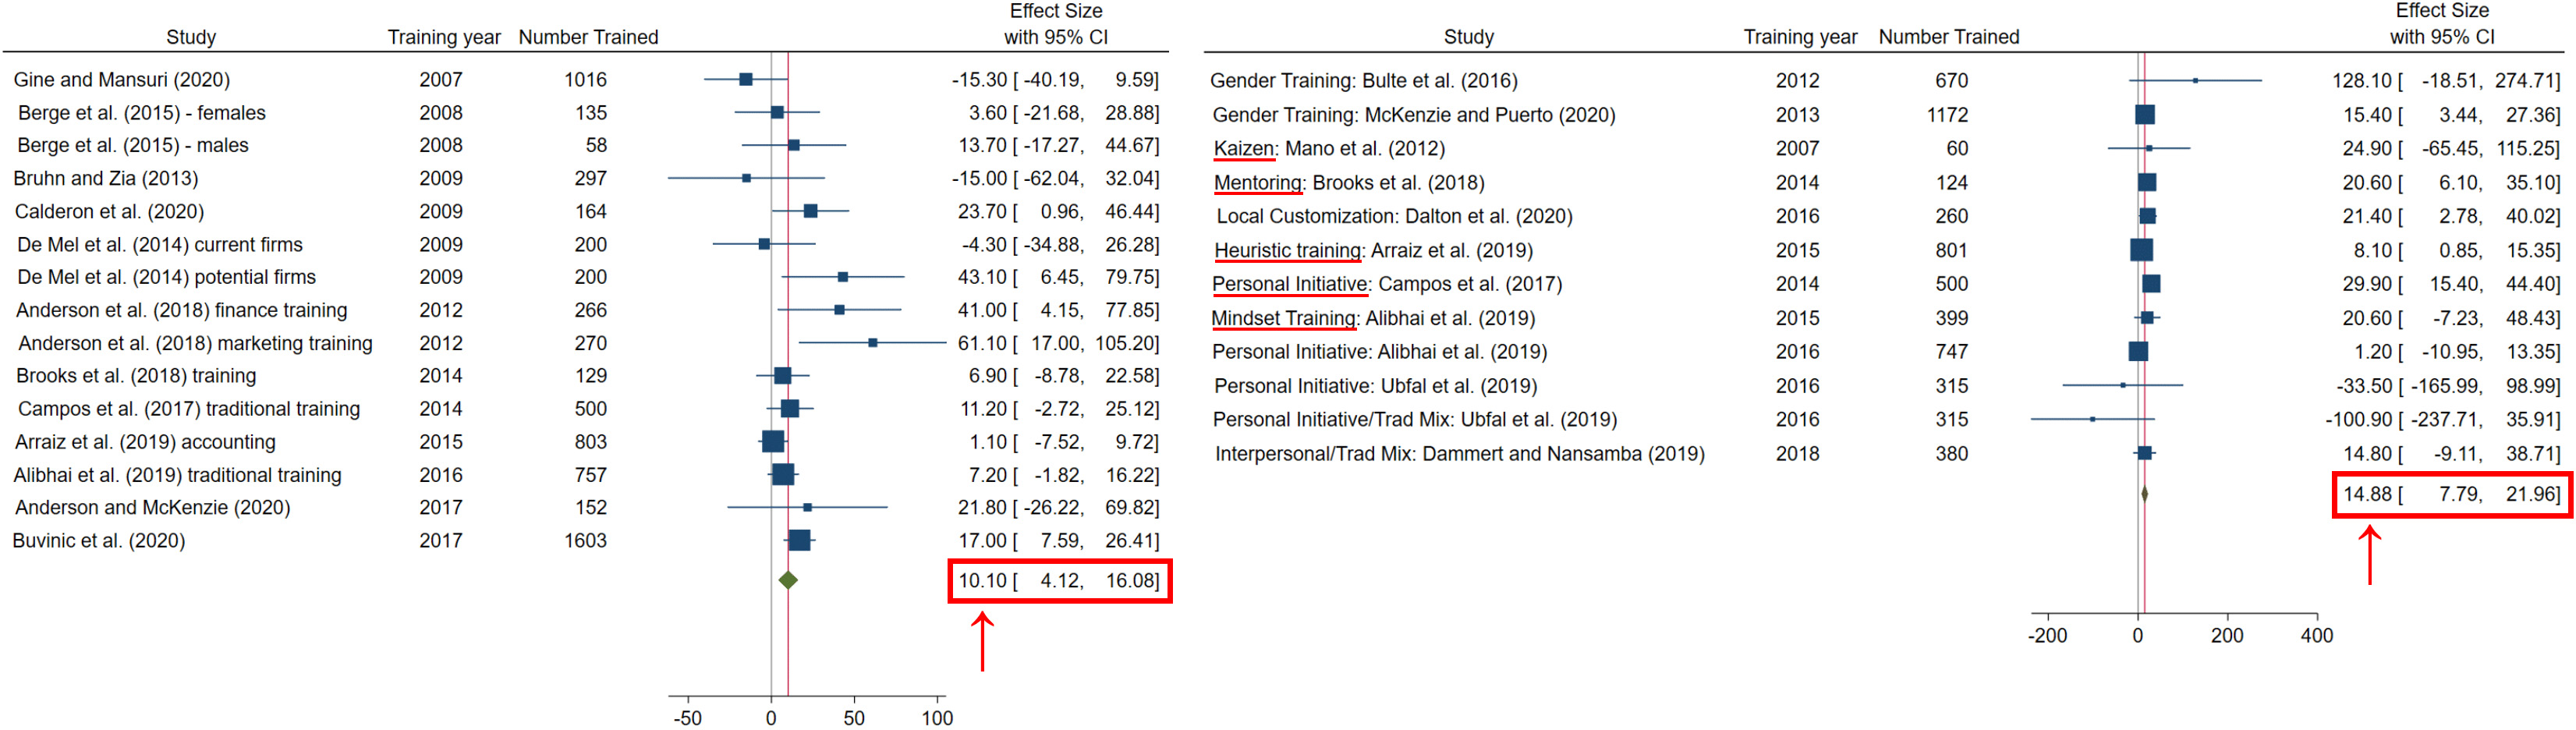
\includegraphics[width=\textwidth]{img/meta-analysis.jpg}
    \label{meta-analysis}
\end{figure}

\section{Including Psychology}

The extensions for the business training programs including psychological insights play an important role and are reviewed by \cite{Frese2014} in "The Psychology of Entrepreneurship". The authors define entrepreneurship as the process of identification and exploitation of business opportunities. A proactive personality drives business success and setting challenging goals yields higher performance over time. Furthermore, they discuss that personal initiative is pivotal throughout the entrepreneurial journey because it helps differentiate the business, create advantages, and achieve better results. Nevertheless, a persistent behavior and a critical and problem-solving attitude are intrinsic to a resilient business.  

All these characteristics can fall under the notion of soft-skills. Researchers have tested whether teaching soft-skills to entrepreneurs can actually improve treatment effects and, if so, through which channels. This is where the work of \cite{Ubfal2022} presented earlier comes in. In their study, they found that entrepreneurs in the soft skills group were more likely (11\%) to experience positive profits than those in combined training (7\%). Although they found that the increase in profits was mainly experienced by men, this change was due to greater adoption of recommended business practices by both men and women. In a similar study, "Teaching personal initiative beats traditional training in boosting small business in West Africa," \cite{Campos2017} demonstrated the effectiveness of such programs. In 2014, they conducted an RCT on 1,500 Togolese microenterprises. One treatment group received classical business training, while the other was taught lessons on developing a proactive entrepreneurial mindset. Similar to \cite{Ubfal2022}, the results supported the initial hypothesis that teaching entrepreneurs soft skills can better influence profits: over the time span of the experiment (2.5 years), monthly profits increased by 30 percent. In contrast to the results of \cite{Ubfal2022}, they found that this increase is experienced by both men and women, but confirmed the adoption of new recommended practices as the main intermediate mechanism. In addition, their results seem to be more persistent throughout the duration of the experiment, which could be due to the participants' monthly visits conducted by a trainer ready to answer any questions and help them implement the principles taught during the training.

\section{Including Mentors}

Another relevant extension to basic business training is the inclusion of mentors assisting the participants.

For instance, in "Business Training and Mentoring: Experimental Evidence from Women-Owned Microenterprises in Ethiopia" by \cite{Bakhtiar2022}, the authors test the effects of regular business training and mentoring for women-owned small firms in Ethiopia. Additionally, in response to the idea that it takes a while for changes in adopted business practices to translate into improved business outcomes, they examine the long-term impacts, up to 3 years after training. The RCT is structured as follows: first, the treatment group is given standard business training; second, the treated participants become mentors and are assigned three randomly selected mentees within their network. Mentors and mentees were asked to meet once a month for six months. While the first training significantly and positively affected participants' revenues and profits, the effects of mentoring on mentees' profits were positive but not significant. However, mentees experienced an increase in the adoption of business practices. In conclusion, \cite{Bakhtiar2022} mainly contributed to demonstrating the power of mentoring as a low-cost tool for transmitting knowledge and practices to improve business outcomes.

\chapter{Extension}
\label{sec:extension}

Let's now delve into some possible extensions or improvements that can be done to the work of \textcite{Larch2017}.

\section{Enhanced Trade Costs Estimates}

As described in Section \ref{sec:theorethical}, since trade costs $T_l^{ij}$ are not directly observable, to measure the trade flows $X_l^{ij}$ between each pair of countries, \textcite{Larch2017} approximate and estimate them using a vector of seven variables. Among others, they include the distance between the two countries or the presence of Bilateral Trade Agreements, and their coefficients (excerpt in Table \ref{tab:tradeFlowEst}) appears to be statistically significant and with a large average Pseudo-$R^2$ of $0.86$.

However, I believe that also another key factor can determine the trade costs between two countries: currency. More precisely, whether both countries officially adopt the same currency nationally. For example, some minor costs could arise from exchanging and storing different currencies or being subject to the volatility of the rates. This hypothesis is further supported by \textcite{Anderson2003}, where they find out that the barriers arising from using different currencies may account up to 14\% of all trade costs. Similarly, analyzing the case of the European Economic and Monetary Union (EMU), \textcite{Andrew2001} highlight the huge positive impact that a common currency can have on reducing trade barriers.

Therefore, using the data of the International Standard ISO 4217, which regulates currency codes worldwide, we can create a dummy variables taking values as follow:
\begin{flalign}
&z^{ij}=
\begin{cases}
1\quad &\textrm{if }currency^i=currency^j\\
0\quad &\textrm{otherwise}
\end{cases}
&
\end{flalign}
where, the variable takes value 1 if both countries adopt the same currency. Now, we can include it in the vector $\boldsymbol{z}_l^{ij}$ of regressors (see Equation \ref{eq:estimate}), and run again the regression for the PPML estimator to estimate the updated measure for trade flows, hopefully now with an even higher $R^2$.

\section{Reinforced Low-Carbon Consumer Preferences}

In Equation \ref{eq:CESutility} (b), \textcite{Larch2017} include in the total utility of the representative consumer a damage factor that reduces utility based on the social cost of carbon $\mu^j$ and the total emissions $E^i$ produced by all other countries, i.e $(\frac{1}{\mu^j}\sum_{i=1}^{N}E^i)^2$.

As it is modeled, pollution is treated as a pure externality and does not directly enter into consumer choice. Nowadays, I believe that consumers actively choose ex-ante a low-carbon consumption bundle, and not only do they suffer the pollution ex-post. This behavior is fostered also by the presence of carbon labels on the products (as highlighted by \textcite{Vanclay2011}), or information regarding the place or production methodology (e.g. bio vs conventional agriculture, recycled vs virgin paper, recycled vs virgin rare earth elements). The two elements work in the same direction and, to my mind, this extension provides an additional micro-foundation to the model.

The new underlying mechanism is as follows: 1) the consumer gains a greater utility from consuming low-carbon goods, 2) therefore, thanks to elasticity in consumption, the expenditure in low-carbon sectors increases and falls in the others, 3) since the balance trade assumption applies, i.e. $Y^j=\mathfrak{X}^j$, everything produced is consumed, a higher share of low-carbon goods is produced, 4) ultimately, the production-share-weighted average energy cost term $\bar{\alpha}^i_E$ is smaller in Equation \ref{eq:emissions}, thus reducing emissions $E^i$. To obtain a closer approximation of this consumption behavior and mechanism, I propose an extension of the utility function previously illustrated in Equation \ref{eq:CESutility} (a).
\begin{flalign}\label{eq:utilityextended}
&U_l^j= \left[\sum_{i=1}^{N}(\beta_l^i)^{\frac{1-\sigma_l}{\sigma_l}}\left(\frac{q_l^{ij}}{\boldsymbol{1+\delta_l^jI_l^{ij}}}\right)^{\frac{\sigma_l-1}{\sigma_l}} \right]^{\frac{\sigma_l}{\sigma_l-1}}
&
\end{flalign}
In Equation \ref{eq:utilityextended} is illustrated the extended utility function. The new parameters are: 1) $\delta_l^j$, which captures the preference for low-carbon intensive goods in sector $l$ and country $j$, 2) $I_l^{ij}$, the carbon intensity of goods from sector $l$ produced in country $i$ and consumed in country $j$.

$\delta_l^j$ serves as a weight: a more environmentalist consumer gives more importance (and weight) to the carbon intensity of the goods she consumes and therefore will have a higher $\delta_l^j$ and, depending on $I_l^{ij}$, a larger denominator, and a lower $U_l^i$. Conversely, an egoist consumer does not value at all carbon intensity, and her $\delta_l^j$ is 0.

$I_l^{ij}$ accounts for the emissions emitted during the production of a unit of a good in country $i$, and is defined as follows: $I_l^{ij}=E_l^i/q_l^i$. Here, when the representative consumer buys a good with a low carbon intensity $I_l^{ij}$, the denominator is smaller, and the utility $U_l^i$ is larger.

In the context of the decomposition analysis of \textcite{Larch2017}, I expect this extension to further increase the composition effect, i.e. $\frac{\delta E^i}{\delta \bar{a}^i_E}$. This effect was already the main driver of emission reductions and now, as consumers have even more incentives to switch to low-carbon consumption, it will increase the share of low-carbon output and, ultimately, reduce emissions. 

In conclusion, besides fulfilling the main role of providing additional micro-foundation, I believe this extension can also correct the often underestimated social cost of carbon. Indeed, a too low estimate of the SCC cannot capture the real damage suffered by the consumer due to pollution and diminishes the attractiveness of a low-carbon consumption bundle. The American Interagency Working Group on the Social Cost of Carbon is the main and most famous research team evaluating such a measure. For instance, \textcite{Larch2017} use a social cost of carbon $\mu^j$ of 29 US-\$ for 2007, in line with \textcite{Nordhaus2017} which uses a SCC of 31 US-\$ for 2010 with a discount rate of 3\%. However, in 2021, while the \textcite{SCC2021} estimated a SCC of 51 US-\$ for 2020, in 2022, \textcite{Rennert2022} estimated a mean SCC of 185 US-\$ per ton of CO2. Still, in 2023, \textcite{SCC2023} found a SCC of 120 US-\$  for 2020 at a $2.5\%$ discount rate. It is clear that the social cost of carbon is constantly evolving, as are the techniques to measure it. Hopefully, this micro-founded extension, together with the disutility factor, can extensively account for the negative impact of carbon emissions.
\chapter{Conclusion}
\label{sec:conclusion}

\textcite{Larch2017} analyze the impacts of introducing carbon tariffs on trade flows, welfare, and emissions effects. Moreover, building on the work of \textcite{copeland2005}, they decompose the forces influencing emissions into three effects: scale, composition, and technique. To this end, they are the first to implement such analysis by exploiting a structural multi-sector and multi-factor gravity model.

Firstly, to address the externalities of carbon emissions, they estimate the consequences of introducing a pure carbon tariff on imports, that is, a tax equal to the carbon tax differential between each pair of countries. They find: 1) global trade flows decrease by 1.9\%, 2) 79\% of the countries experiences a welfare loss, and developing countries suffer the most, 3) however, world carbon emissions decrease by 0.50\%. Breaking down the forces behind the change in emissions, they reveal that the main driver is the composition effect, which means that low-carbon sectors have increased their share in global production.

Secondly, they estimate once again the impacts of carbon tariffs on trade, welfare, and carbon emissions, in case a subgroup of countries (Annex I from the Kyoto Protocol) fully reaches its climate pledges. The goal is to explain whether carbon tariffs can also reduce carbon leakage, a major problem when it comes to meeting the targets of international agreements. They point out that: 1) in the case where the Annex I group reaches its pledges but carbon tariffs are not in place, carbon leakage amounts to 13.4\%, and emissions decrease by 8.4\%, 2) on the other hand, with carbon tariffs, carbon leakage falls to 4.14\%, and emissions shrink by 9.3\%.
\chapter*{Bibliography}
\addcontentsline{toc}{chapter}{Bibliography}

%\section*{Book references}

%\begingroup
%\let\clearpage\relax
%\printbibliography[type=book,heading=none]
%\endgroup

\section*{Article references}

\begingroup
\let\clearpage\relax
\printbibliography[type=article,heading=none]
\endgroup

\end{document}